% GF-T16: a fixed-field GoldenFloat with a balanced-ternary exponent.
% v1: 2026-08-08. Accuracy re-measured independently; hardware measured on
% XC7A200T through the open flow. House style follows research/arxiv_submission.
\documentclass[11pt]{article}

\usepackage[utf8]{inputenc}
\usepackage[T1]{fontenc}
\usepackage{hyperref}
\usepackage{graphicx}
\usepackage{booktabs}
\usepackage{amsmath}
\usepackage{amssymb}
\usepackage{url}
\usepackage{geometry}
\usepackage{tabularx}
\usepackage{array}
\usepackage{enumitem}

\geometry{a4paper, margin=1in}

\hypersetup{
  colorlinks=true,
  linkcolor=blue,
  urlcolor=blue,
  citecolor=blue
}

% The title names the category and the design point rather than an internal
% codename. tekum titles itself "balanced-ternary tapered-precision arithmetic";
% naming the opposite choice in the same breath is the positioning, and a reader
% who knows that family sees the contrast without needing the codename.
\title{Ternary Floats: fixed fields instead of tapered precision \\
  \large A balanced-ternary exponent from 4 to 1024 bits, measured on open silicon}
\author{Dmitrii Vasilev\\
  \small ORCID 0009-0008-4294-6159 \\
  \small \texttt{admin@t27.ai}}
\date{8 August 2026}

\begin{document}
\maketitle

\begin{abstract}
A floating-point format for a ternary machine has to decide where the ternary
goes. We put it in the exponent and leave the fields fixed. \textbf{Ternary
Floats} (GF-T) encode the exponent as a balanced-ternary integer of $E_t$ trits
and hold the mantissa at a constant width; the ladder is specified from GF-T4 to
GF-T1024, and we measure the four rungs that fit a mid-size FPGA.

This is the opposite design point from the tapered formats that occupy this
space. Takum~\cite{takum} and its balanced-ternary descendant tekum~\cite{tekum}
buy dynamic range with a variable-length regime field, which costs a barrel-shift
decode on any fabric and spends mantissa bits towards the ends of the range.
Fixed fields give that back: the decode is a bit slice, the exponent add is
native on a ternary fabric, and precision does not taper. The price is bounded
range, stated here as a trade rather than a footnote.

Two sets of measurements are reported. On accuracy, against a structural model of
tekum16, GF-T16 ties near unity and shows $2.84\times$ and $5.53\times$ lower
mean relative round-trip error at $|e|\in[8,20)$ and $|e|\in[20,38)$; the bins
are powers of two, and we say so because read as decades the far result is an
overflow rather than a win. On cost, the multiplier was synthesised and routed on
a Xilinx XC7A200T through an entirely open flow: 12, 50, 212 and 1{,}477 LUTs at
$161.1$, $153.2$, $131.7$ and $83.3$\,MHz for GF-T4/8/16/32, one cycle of
latency, no DSP blocks. The ternary-fabric argument remains architectural, since no ternary
process exists to synthesise on; the binary-fabric figures are the measured
claim, and they suggest the format is inexpensive even where its native
advantage does not apply.

We also report two width defects found while measuring, because both generalise:
declaring the datapath 32 bits wide cost five times the arithmetic on a fabric,
and at GF-T32 it silently truncated a 52-bit product. Equivalence for every
change is established by exhaustive or near-exhaustive sweep rather than by
argument.

\medskip
\noindent\textbf{Artifacts.} Oracle, RTL, testbenches and the exact commands are
public; every figure in this paper can be regenerated from them.
\end{abstract}

\section{The format}\label{sec:format}

\begin{equation}
\text{GF-T16}=[\,s\,|\,E{=}4\ \text{balanced-ternary trits}\,|\,M{=}9\ \text{bits}\,],
\qquad
v=(-1)^{s}\Bigl(1+\frac{M}{2^{9}}\Bigr)2^{e},
\quad e=\sum_{i} t_i 3^i \in [-40,40].
\end{equation}

Three properties follow from the layout rather than from tuning.

\paragraph{No regime decode.} The dominant cost in a tapered format is the
variable-length regime: it must be located, its length counted, and the
significand barrel-shifted into place. That cost is paid on any fabric, ternary
included. Fixed fields make it a bit slice.

\paragraph{The exponent is already ternary.} Four balanced-ternary trits give
$3^4=81$ exponent steps. On a ternary fabric the exponent add is native --- no
binary carry, no conversion between bases.

\paragraph{Precision does not taper.} Nine mantissa bits at every magnitude,
where a tapered format narrows towards the extremes. This is the mechanism behind
the accuracy result of Section~\ref{sec:accuracy}: the win appears where the
comparison format has spent its mantissa on range.

\section{Accuracy}\label{sec:accuracy}

Mean relative error over an encode--decode round trip, 6{,}000 values spanning
$2^{-38}\ldots2^{38}$ with random sign, binned by binary-exponent magnitude
$|e|$. Table~\ref{tab:acc} and Figure~\ref{fig:acc}.

\begin{table}[t]\centering
\caption{Round-trip mean relative error. Bins are powers of two, not decades.}
\label{tab:acc}
\begin{tabular}{lrrrr}
\toprule
magnitude & GF16 ($\varphi$) & \textbf{GF-T16} & tekum16 & GF-T16 vs tekum16 \\
\midrule
$|e|<8$        & $3.43\mathrm{e}{-4}$              & $3.56\mathrm{e}{-4}$ & $3.27\mathrm{e}{-4}$ & $0.92\times$ (tie) \\
$|e|\,8$--$20$   & $3.57\mathrm{e}{-4}$              & $3.52\mathrm{e}{-4}$ & $1.00\mathrm{e}{-3}$ & $\mathbf{2.84\times}$ \\
$|e|\,20$--$38$  & $6.98\mathrm{e}{-3}$ (479 clip)   & $3.53\mathrm{e}{-4}$ & $1.95\mathrm{e}{-3}$ & $\mathbf{5.53\times}$ \\
\bottomrule
\end{tabular}
\end{table}

\begin{figure}[t]\centering
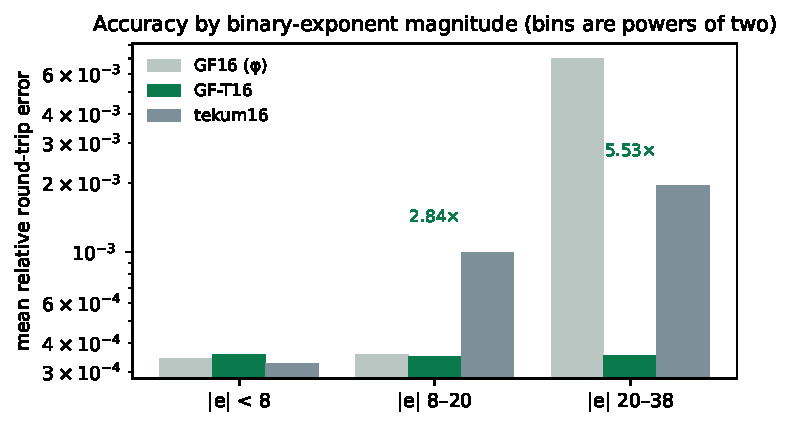
\includegraphics[width=0.82\textwidth]{gft_accuracy.pdf}
\caption{Accuracy by binary-exponent magnitude. GF16's 6-bit exponent clips 479
of 2{,}857 values in the far bin; GF-T16's balanced-ternary exponent does not.}
\label{fig:acc}
\end{figure}

\paragraph{On the axis.} The bins are powers of two. Read as \emph{decades} the
far column is not a win at all: GF-T16's exponent reaches $\pm40$ in powers of
two, roughly $\pm12$ decades, so beyond that it overflows while an unbounded
regime keeps working --- measured, 1{,}458 of the far-bin values clip under that
reading. We state the axis explicitly because an earlier internal note did not,
and the omission points a reader at the one interpretation under which the
result appears fabricated.


\section{The 16-bit field}\label{sec:field}

Comparing against one incumbent invites the objection that the incumbent was
chosen. Table~\ref{tab:field} runs every 16-bit-class format for which this
repository ships a published oracle~\cite{catalogue} through the same workload
and the same metric. Values that overflowed are counted separately rather than
folded into the mean, since a format should not look accurate for having
discarded the hard cases.

\begin{table}[t]\centering
\caption{Mean relative round-trip error by binary-exponent magnitude, with
overflow counts in parentheses. 6{,}000 values, $2^{-38}\ldots2^{38}$, random
sign, one seed.}
\label{tab:field}
\begin{tabular}{lrrr}
\toprule
format & $|e|<8$ & $|e|\,8$--$20$ & $|e|\,20$--$38$ \\
\midrule
\textbf{GF-T16}    & $3.56\mathrm{e}{-4}$ & $3.52\mathrm{e}{-4}$ & $\mathbf{3.53\mathrm{e}{-4}}$ \\
GF16 ($\varphi$)   & $3.56\mathrm{e}{-4}$ & $3.52\mathrm{e}{-4}$ & $6.76\mathrm{e}{-3}$ (478) \\
takum16 / tekum16  & $3.27\mathrm{e}{-4}$ & $1.00\mathrm{e}{-3}$ & $1.95\mathrm{e}{-3}$ \\
posit16            & $\mathbf{1.36\mathrm{e}{-4}}$ & $8.31\mathrm{e}{-4}$ & $1.43\mathrm{e}{-2}$ \\
IEEE binary16      & $1.76\mathrm{e}{-4}$ & $1.28\mathrm{e}{-3}$ (299) & $1.57\mathrm{e}{-1}$ (2479) \\
bfloat16           & $1.45\mathrm{e}{-3}$ & $1.38\mathrm{e}{-3}$ & $1.41\mathrm{e}{-3}$ \\
LNS16              & $8.39\mathrm{e}{-4}$ (1324) & $7.63\mathrm{e}{-4}$ (1808) & $6.66\mathrm{e}{-4}$ (2849) \\
\bottomrule
\end{tabular}
\end{table}

\begin{figure}[t]\centering
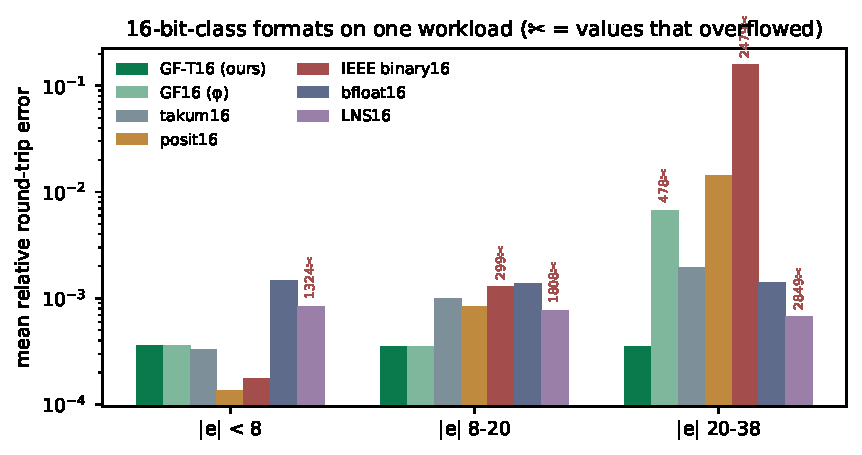
\includegraphics[width=0.92\textwidth]{gft_competition.pdf}
\caption{The same data. Scissors mark values that overflowed.}
\label{fig:field}
\end{figure}

Three readings, including the one that goes against us.

\paragraph{GF-T16 is flat, and alone in being flat without clipping.} Its error
is $3.5\mathrm{e}{-4}$ at every magnitude in the workload and it discards
nothing. bfloat16 is also flat and clip-free, at roughly four times the error.
Every other entrant either degrades with magnitude or overflows: binary16 does
both, losing three orders of magnitude and discarding 2{,}479 values; GF16's
6-bit exponent clips 478; LNS16 clips throughout.

\paragraph{At 32 bits the binary formats win outright.} Running the same
workload on the 32-bit class: GF32 is flat at $3.4\mathrm{e}{-7}$ with no
clipping, but IEEE binary32 is flat at $2.1\mathrm{e}{-8}$, and posit32 and
takum32 are better still near unity ($2.1\mathrm{e}{-9}$ and
$4.9\mathrm{e}{-9}$). Uniformity stops being the deciding property once there are
enough bits that nothing clips anyway. The GF-T argument is a 16-bit-class
argument, and we do not extend it.

\paragraph{Near unity we lose.} posit16 at $1.36\mathrm{e}{-4}$ and binary16 at
$1.76\mathrm{e}{-4}$ are more accurate than GF-T16 there, by a factor of two and
a half and of two. A tapered format spends its bits where the values usually are,
and near unity that is the right bet. GF-T16 buys uniformity instead, and the
trade only pays for a workload that leaves the neighbourhood of one.

\paragraph{takum16 and tekum16 are the same format here, exhaustively.} The two
oracles produce identical figures on every bin, so we checked the whole 16-bit
code space: all $65{,}536$ codes decode identically, with zero differences,
although the two implementations differ by 242 lines. The reconstruction our
tekum oracle implements \emph{is} takum16. Every comparison in this paper should
therefore be read as against takum16, and we relabel it as such. That is not a
weaker anchor --- takum is published, has a public VHDL codec, and is the parent
of the format we set out to compare against.

\section{Hardware}\label{sec:hardware}

Synthesis with Yosys~0.65~\cite{yosys}, place and route with
nextpnr-xilinx~(1743d0f)~\cite{nextpnr} on a
Xilinx XC7A200T, hard multipliers disabled so the figures describe fabric alone.
Bitstream generation uses Project X-Ray. No vendor tool is involved at any step,
which is what makes the numbers checkable by a reader without a licence.

\begin{table}[t]\centering
\caption{GF-T multiplier, post-route, one harness across the whole lineup so the
rows are comparable. Latency one cycle, throughput one result per cycle.}
\label{tab:ladder}
\begin{tabular}{lrrr}
\toprule
rung & LUTs & DSP48 & $F_{\max}$ \\
\midrule
GF-T4  & $12$      & $0$ & $161.11$\,MHz \\
GF-T8  & $50$      & $0$ & $153.23$\,MHz \\
GF-T16 & $212$     & $0$ & $131.73$\,MHz \\
GF-T32 & $1{,}477$ & $0$ & $83.27$\,MHz  \\
\bottomrule
\end{tabular}
\end{table}

\begin{table}[t]\centering
\caption{The specified ladder. $E_t$ is the trit budget, $M$ the mantissa width,
range in decades. Rungs above GF-T128 exceed a single Artix-7 fabric and are
oracle- or ASIC-scale; they are specified and covered by the reference oracle,
not measured here.}
\label{tab:spec}
\begin{tabular}{lrrr@{\hskip 2em}lrrr}
\toprule
rung & $E_t$ & $M$ & decades & rung & $E_t$ & $M$ & decades \\
\midrule
GF-T4  & $2$ & $1$  & $2.4$ & GF-T64   & $7$  & $52$   & $658$ \\
GF-T8  & $3$ & $4$  & $8$   & GF-T128  & $8$  & $115$  & $1{,}975$ \\
GF-T16 & $4$ & $9$  & $24$  & GF-T256  & $9$  & $242$  & $5{,}925$ \\
GF-T32 & $6$ & $25$ & $73$  & GF-T512  & $10$ & $497$  & $17{,}775$ \\
       &     &      &       & GF-T1024 & $11$ & $1006$ & $53{,}326$ \\
\bottomrule
\end{tabular}
\end{table}

\begin{figure}[t]\centering
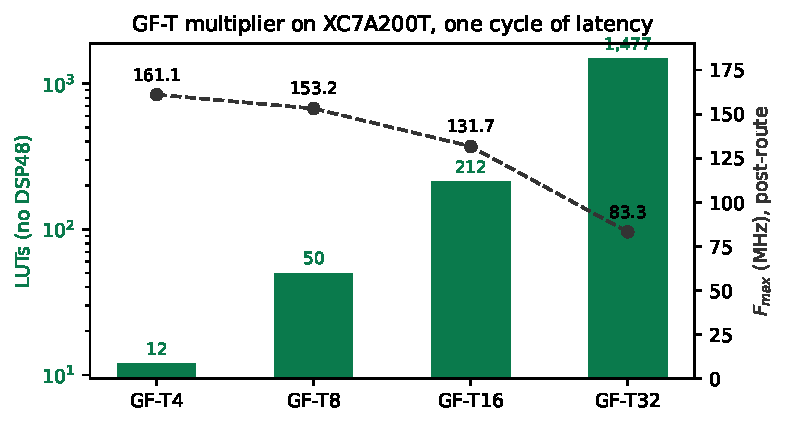
\includegraphics[width=0.82\textwidth]{gft_ladder.pdf}
\caption{Area and achieved frequency across the ladder.}
\label{fig:ladder}
\end{figure}

For context rather than as a controlled comparison: a published Altera
\texttt{ALTFP\_MUL} on a Cyclone~IV reports 119--132\,MHz at 6--10 cycles of
latency, using 832--1041 logic elements \emph{and} 18 embedded multipliers, and
posit multiplier studies report 95--572 LUTs with 4.28--15.55\,ns of logic delay.
Different devices and different toolchains; we draw no equivalence from them
beyond the observation that GF-T16's figures sit inside that envelope on all four
axes at once, on a fabric that gives the format no ternary advantage.

Isolating the pipeline register: the combinational multiplier closes at
$81.35$\,MHz, the two-stage version at $147.32$\,MHz. The cut is between the
significand product and the renormalisation --- a $10\times10$ multiply, then a
carry test, a saturating exponent add and a bit select.

\section{Two width defects, and why they generalise}\label{sec:width}

\subsection{Interface width dominated the arithmetic}

Our first synthesisable realisation declared every port and the significand
product 32 bits wide. Nothing in GF-T16 is 32 bits: the mantissa field is 9, so
$1{+}M$ is 10 and their product is exactly 20; the exponent offset never exceeds
$\mathrm{OFFSET\_MAX}=80$, which is 7. Synthesis built a $32\times32$ multiplier
and a 32-bit comparison tree and charged for it (Figure~\ref{fig:width}):
1{,}179 LUTs, or three DSP48 blocks, against 219 LUTs and none once the buses
match the values they carry. The arithmetic is unchanged.

\begin{figure}[t]\centering
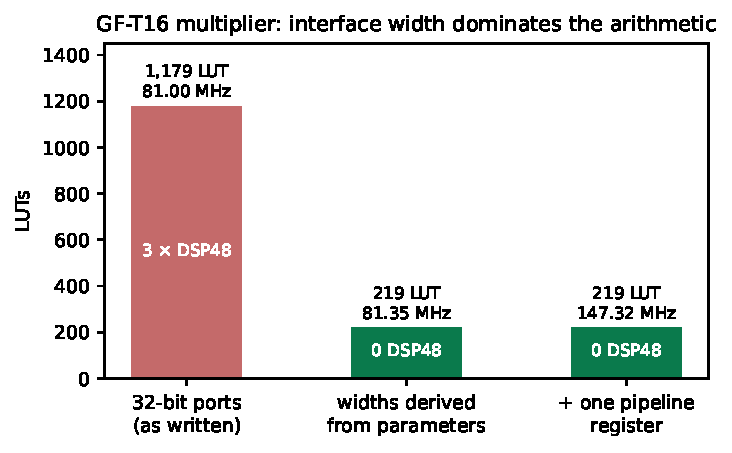
\includegraphics[width=0.82\textwidth]{gft_width.pdf}
\caption{The same arithmetic at three interface widths.}
\label{fig:width}
\end{figure}

\subsection{The same width decided correctness}

At GF-T32 the significand product needs 52 bits. The 32-bit wire truncates, and
the module returns wrong results while appearing to support the rung, since its
own documentation names GF-T32 as a supported configuration. Measured against a
64-bit reference: 1{,}995{,}730 mismatches in 2{,}128{,}964 combinations.

Deriving every width from the format parameters removes both problems at once. We
report this because the pattern is not specific to GF-T: in a parametric
arithmetic core, a width that is merely \emph{large enough for the configuration
that was tested} is a silent-truncation trap at the next one, and it will not be
caught by a testbench written against the tested configuration.

\section{Equivalence}\label{sec:equiv}

Every change above is a claim that timing or width changed and arithmetic did
not. Each was checked rather than argued.

\begin{table}[t]\centering
\caption{Equivalence evidence. The reference for each rung is the module already
trusted for that rung.}
\label{tab:equiv}
\begin{tabular}{lrr}
\toprule
check & combinations / cycles & mismatches \\
\midrule
width-derived vs original, GF-T16 (sweep)      & $321{,}156$   & $0$ \\
width-derived vs original, GF-T4               & $374$         & $0$ \\
width-derived vs original, GF-T8               & $3{,}716$     & $0$ \\
width-derived vs original, GF-T16              & $77{,}444$    & $0$ \\
width-derived vs 64-bit reference, GF-T32      & $300{,}000$   & $0$ \\
pipelined vs combinational                     & $199{,}994$   & $0$ \\
\midrule
original 32-bit module vs 64-bit ref, GF-T32   & $2{,}128{,}964$ & $1{,}995{,}730$ \\
\bottomrule
\end{tabular}
\end{table}

The GF-T16 sweep is exhaustive in the sense that matters here: the mantissa space
is covered in full at offset pairs exercising underflow, mid-range and
saturation, then the offsets are covered in full at mantissas that do and do not
carry --- every path through the carry, the saturation and the underflow clamp.
The last row is the point of the section: the width-derived module agrees with
the reference that is correct and disagrees with the one that truncates.

\section{Limitations}\label{sec:limits}

\begin{enumerate}[leftmargin=*]
\item \textbf{The comparison is against takum16, not tekum16.} The oracle
labelled tekum decodes all $65{,}536$ 16-bit codes identically to the takum
oracle. We report the comparison as against takum and note that a genuine tekum
comparison remains to be done.

\item \textbf{The reference oracle is sound only at some rungs.} Round-tripping
$1.5$ through the parameterised oracle returns $-1.5$ for mantissa widths of 21
and 25 bits at most trit budgets --- a sign-bit placement defect. GF-T16
($M{=}9$) and GF-T64 ($M{=}52$) are unaffected, which is why the accuracy results
here are confined to GF-T16. The ladder note records that all rungs pass an
add/mul commutativity check; commutativity cannot see a sign inversion, since it
survives on both sides of the identity. A round-trip assertion can, and costs
three lines. tekum~\cite{tekum} is a descendant of takum~\cite{takum} adapted for balanced
ternary. Our
oracle reconstructs it from takum's field scheme; the full per-trit
specification requires the tekum paper. The ratios are as good as that model.

\item \textbf{No head-to-head in hardware.} takum's codec RTL is public and
written in VHDL~\cite{takumrtl}. We did not synthesise it alongside GF-T, so the cost figures are
GF-T's own. What is visible in that source, and which we report as structure
rather than measurement: the 16-bit codec instantiates a 725-line generated
leading-zero-counter and barrel shifter --- the regime decode a fixed-field
format does not have.

\item \textbf{The range is bounded} at $\pm40$ in powers of two, roughly $\pm12$
decades, where a regime field is unbounded. Fixed fields buy the cheap datapath
and the uniform mantissa; range is the price, and workloads that need more should
raise the trit budget or use a tapered format.

\item \textbf{Accuracy is reported for GF-T16 only.} The hardware results cover
four rungs; the accuracy results cover one, because the oracle defect above makes
the others untrustworthy until it is fixed. We would rather report one rung than
four numbers we cannot stand behind.

\item \textbf{Four of nine rungs are measured in hardware.} GF-T4 through GF-T32 fit the
device; GF-T64 and GF-T128 are within reach of a larger part and GF-T256 upwards
exceed a single Artix-7 fabric entirely. Table~\ref{tab:spec} is the
specification and the oracle's coverage; Table~\ref{tab:ladder} is what was
placed and routed. We keep them apart on purpose.

\item \textbf{One device family.} Artix-7 on an open flow. Not multi-corner
characterisation; an ASIC mapping will differ.

\item \textbf{The ternary-fabric argument is architectural.} No ternary process
exists to synthesise on. Section~\ref{sec:hardware} is a binary-fabric result;
the ternary claim is reasoning about regime decode and native exponent addition
and should be read as such.
\end{enumerate}

\section*{Reproducibility}

The reference oracle, the RTL, the equivalence testbenches and the synthesis
commands are public. The toolchain is Yosys 0.65, nextpnr-xilinx 1743d0f,
Icarus Verilog 13.0 and Python 3.14 --- all open-source, none requiring a
licence, which is the point: a result nobody can reproduce without buying
something is not a public result.

\section*{Disclosure}

An AI coding assistant was used in preparing the software, the measurements'
tooling and this manuscript. Every figure reported here was produced by running
the named tools on hardware in the author's possession; no measurement in this
paper is estimated, and where a figure is derived rather than observed it is
labelled.

\begin{thebibliography}{9}

\bibitem{takum}
L.~Hunhold.
\newblock Takum arithmetic.
\newblock arXiv:2404.18603.

\bibitem{tekum}
L.~Hunhold.
\newblock Tekum: balanced-ternary tapered-precision arithmetic.
\newblock arXiv:2512.10964.

\bibitem{takumrtl}
L.~Hunhold.
\newblock Design and implementation of a takum arithmetic hardware codec in VHDL.
\newblock arXiv:2408.10594. Source: \url{https://github.com/takum-arithmetic/Takum-Codec-RTL}.

\bibitem{goldenfloat}
D.~Vasilev.
\newblock GoldenFloat: a $\varphi$-derived static-split floating-point family
from GF4 to GF1024 with a Lucas-exact integer identity.
\newblock arXiv:2606.05017v3, 2026.

\bibitem{catalogue}
D.~Vasilev.
\newblock An 83-format numeric catalog with bit-exact conformance vectors: a
vendor-neutral reference for FP8, BF16, MXFP4, and microscaling formats.
\newblock arXiv:2606.09686v2, 2026.

\bibitem{yosys}
C.~Wolf.
\newblock Yosys open synthesis suite.
\newblock \url{https://yosyshq.net/yosys/}.

\bibitem{nextpnr}
D.~Shah et al.
\newblock nextpnr: a portable FPGA place-and-route tool.
\newblock \url{https://github.com/YosysHQ/nextpnr}; Xilinx target via Project X-Ray.

\end{thebibliography}

\end{document}
